\documentclass{article}
\usepackage{graphicx}
\usepackage{amsmath}
\usepackage{amsfonts}
\usepackage{bookmark}
\usepackage{booktabs}
\usepackage{exercises}
\graphicspath{ {./images/4.3} }
\usepackage{indentfirst}
\usepackage{amsthm}
\usepackage{yhmath}
\usepackage{placeins}
\newcommand*{\oldneg}{\mathord{\sim}}
\newcommand\showdiv[1]{\overline{\smash{)}#1}}
\newcommand\Mydiv[1]{%
\smash{\raise.3ex\hbox{$\big)$}}\mkern-8mu
        \overline{\enspace\strut#1}}
\setlength{\tabcolsep}{5pt}
\theoremstyle{definition}
\newtheorem{definition}{Definition}

\setlength{\parindent}{.5in}
\setlength{\parskip}{12pt}
\renewcommand{\arraystretch}{2}
\newcommand{\?}{\stackrel{?}{=}}

\title{4.3 Answers}
\begin{document}
\maketitle

\section*{1}
The number $e$ is an irrational number approximately equal to 2.71828.

\section*{2}
A natural base exponential function $y=ae^{rx}$ is an exponential growth function if $a>0,r>1$, and is an exponential decay function if 
$a>0,r<1$. In the given example, $r=4$, meaning this is an exponential growth function.

\section*{11}
\[ \frac{3e}{e^x}=3e^{1-x} \]

\section*{12}
\[ \frac{4e^x}{e^{4x}}=4e^{-3x}=\frac{4}{e^{3x}} \]

\section*{13}
\[ \sqrt[3]{8e^{9x}}=2e^{3x} \]

\section*{14}
\[ \frac{6e^{4x}}{8e}=\frac{3e^{4x-1}}{4} \]

\section*{15}
\[ (4e^{2x})^3=64e^{6x} \] C

\section*{16}
\[ \sqrt{\frac{4(27e^{13}x)}{3e^7x^{-3}}} \] \[ =\sqrt{36e^6x^4}=6e^3x^2\]
D

\section*{17}
The error here is that the answer incorrectly used the power of a product property. Instead, the $2$nd power of $3$ should have also been applied:
\[ (3e^{5x})^2=3^2\times e^{5x\times 2}=9e^{10x} \]

\section*{29}
\[ -6e^{2.4}\approx -66.14 \]

\section*{30}
\[ 0.4e^{4.1}\approx 24.14 \]

\section*{35}
Exponential decay.

\section*{36}
Exponential growth.

\section*{37}
Exponential growth.

\section*{38}
Exponential decay.

\section*{39}
B

\section*{40}
C

\section*{41}
A

\section*{52}
$e$ cannot be expressed as a ratio between two integers, as $e$ is an irrational number; by definition, an irrational number cannot be expressed as a 
ratio between two integers.

\section*{53}
We need both $f$ and $g$ to be exponential decay functions, meaning both $r$ and $q$ are less than 0. One such example where 
$\frac{f(x)}{g(x)}$ is an exponential growth function is:
\[ f(x)=10e^{-0.5x},g(x)=2e^{-1.5x} \] meaning \[ \frac{f(x)}{g(x)}=\frac{10e^{-0.5x}}{2e^{-1.5x}}=5e^{x} \]

\section*{54}
Suppose that $A=P\left( 1+\frac{r}{n}\right)^{nt}$. We wish to show that it approaches $Pe^{rt}$ as $n\rightarrow +\infty$. We can evaluate the limit 
as $m\rightarrow +\infty$ where $m=\frac{n}{r}$, meaning $m\rightarrow +\infty$ as $n\rightarrow +\infty$:
\[ \lim_{m\rightarrow +\infty}\left(P\left( 1+\frac{1}{m}\right)^{mrt}\right) \]
\[ =P\lim_{m\rightarrow +\infty}\left( \left(1+\frac{1}{m}\right)^{mrt}\right) \]
\[ =P\left(\lim_{m\rightarrow +\infty} \left( (1+\frac{1}{m})^m\right)\right)^{rt} \]
\[ =Pe^{rt} \] by the assumption of the value of $e$, thus proving the hypothesis.

\section*{58}
We are given a principal amount of $\$800$, and a $2.65\%$ annual interest compounded continuously. Thus, a model to find the balance after $t$ years is:
\[ A=800e^{0.0265t} \] meaning, after $12.5$ years, the balance will be:
\[ A=800e^{0.0265(12)}\approx \$1099.50 \]

\section*{62}
(a): \newline 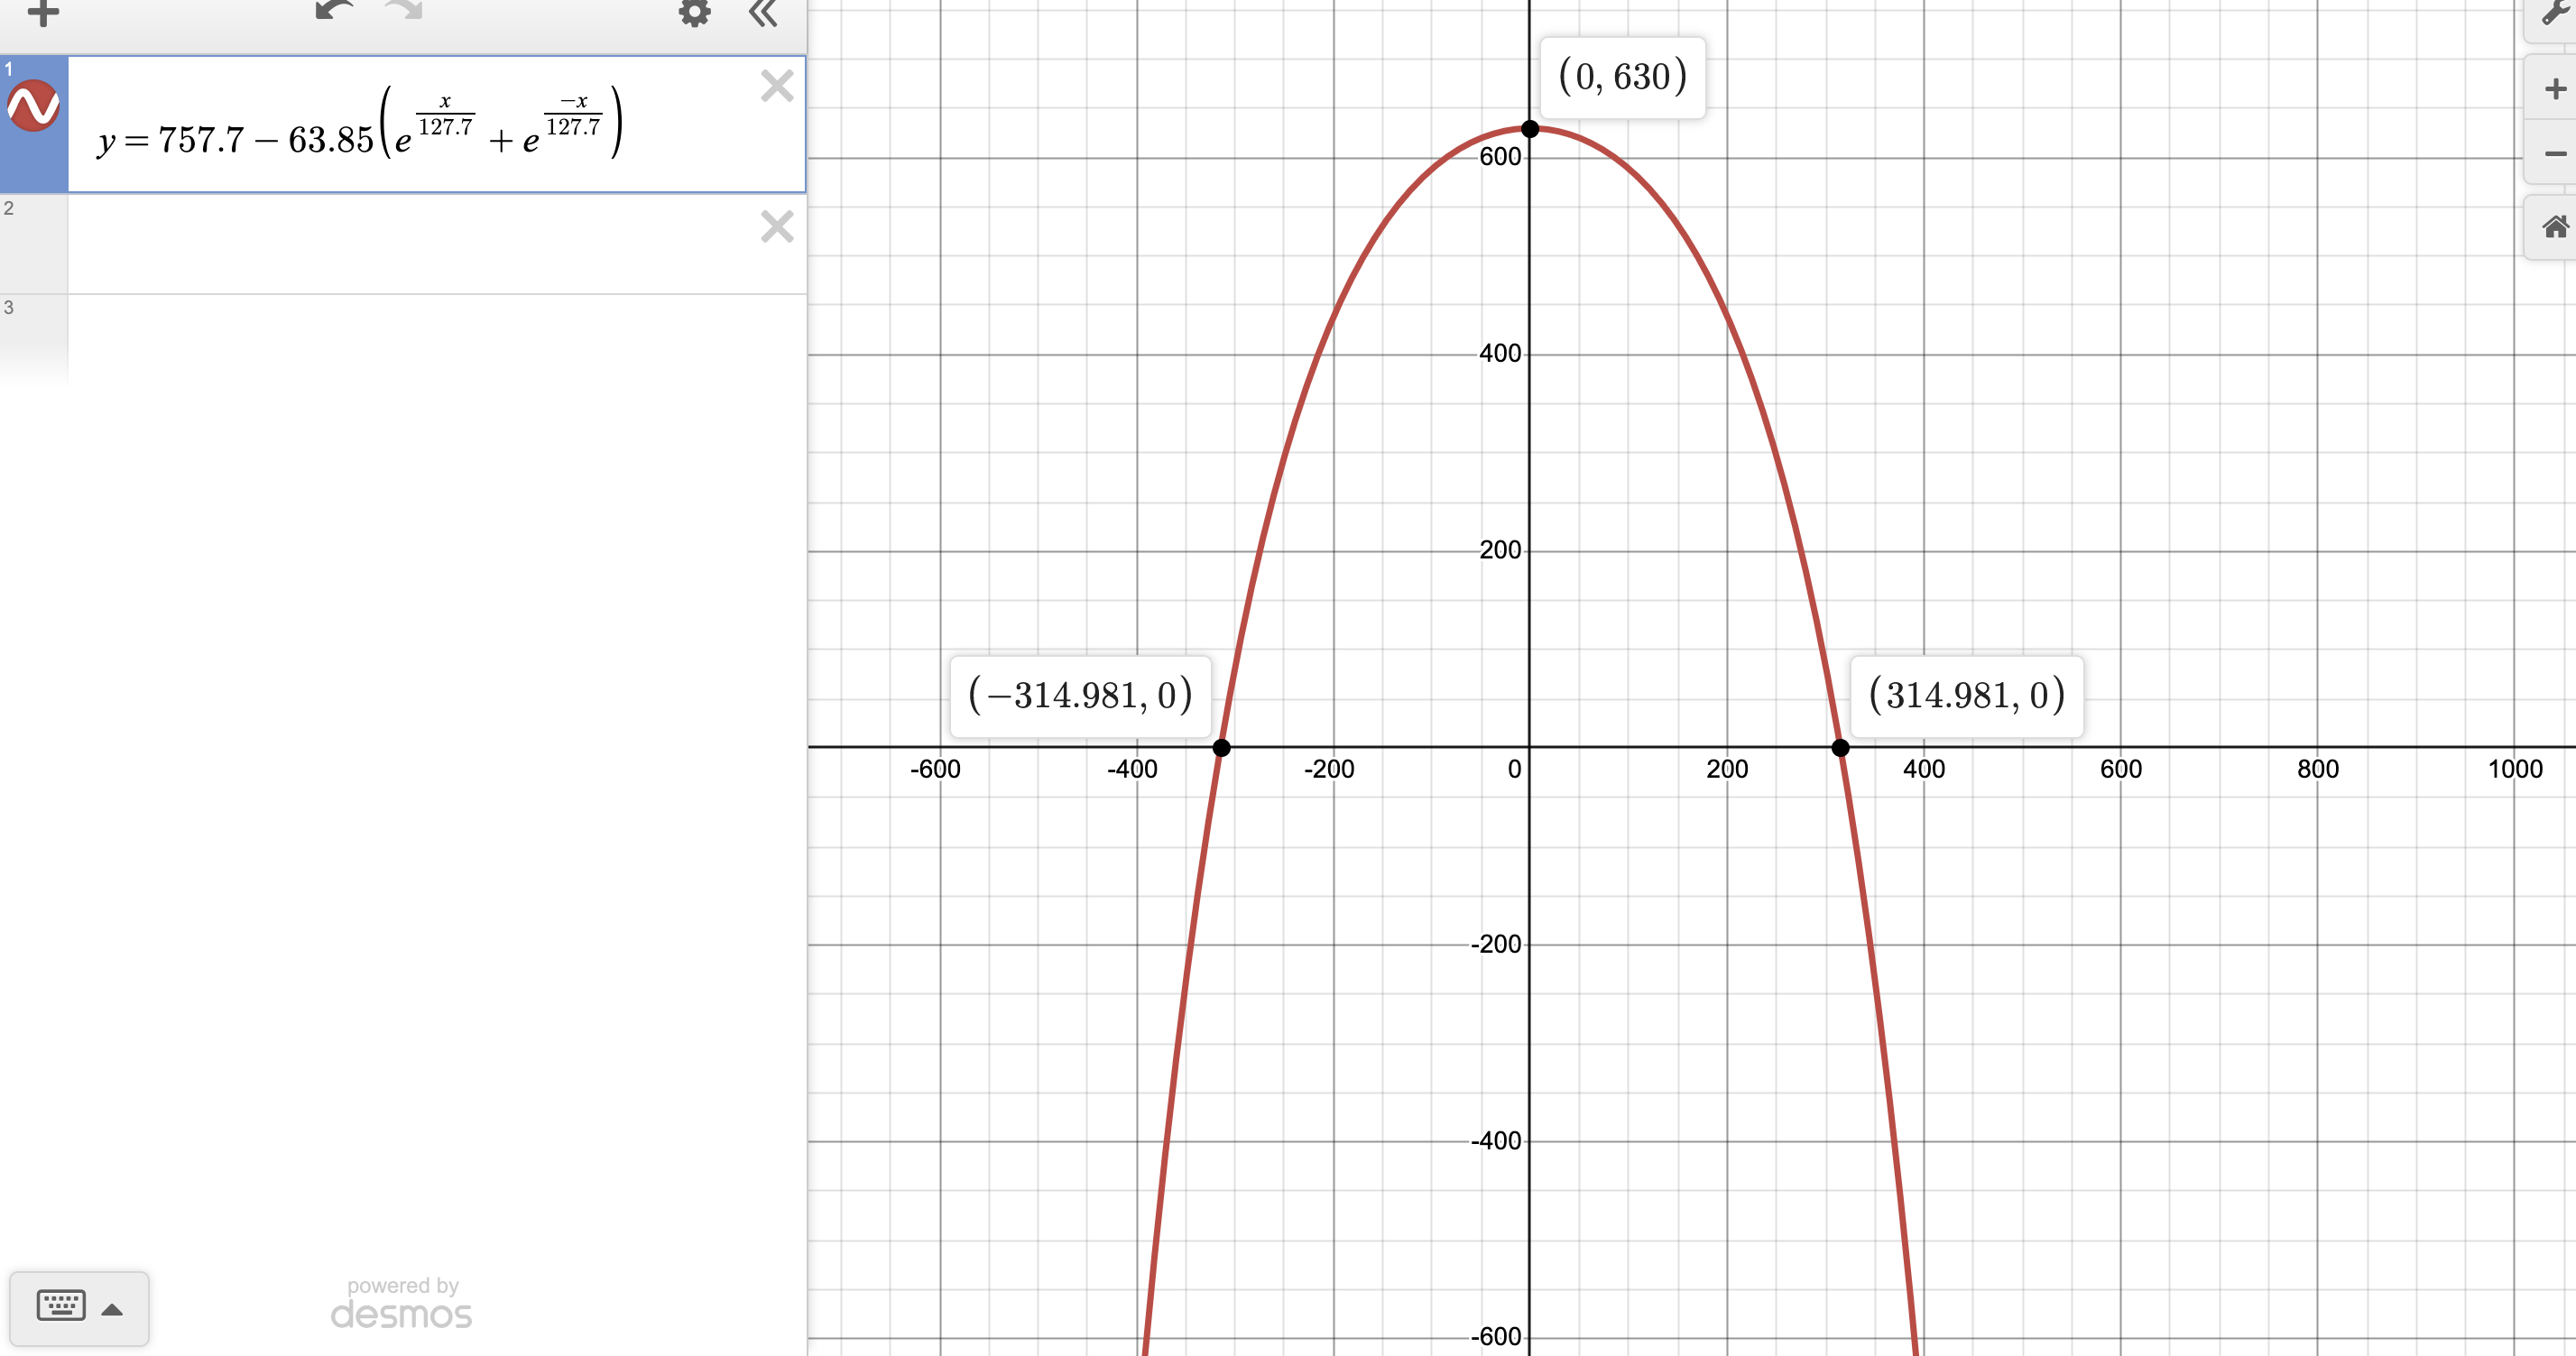
\includegraphics[width = 4in, height = 4in]{62}\newline The arch is 630 feet tall at its highest point.\newline
(b): The ends of the arch are about $314.981+314.981=629.962$ feet apart.

\end{document}
